%%%%%%%%%%%%%%%%%%%%%%%%%%%%%%%%%%%%%%%%%%%%%%%%%%%%%%%%%%%%%%%%%%%%%%%%%%%%
\documentclass[a4j]{jarticle}

\usepackage{jsaisig}
\usepackage[dvipdfmx]{graphicx}

%%%%%%%%%%%%%%%%%%%%%%%%%%%%%%%%%%%%%%%%%%%%%%%%%%%%%%%%%%%%%%%%%%%%%%%%%%%

\begin{document}

% 和文タイトル
\title{ソフトウェア工学}

\author{E1237 森 篤史}


\maketitle
\thispagestyle{empty}

%%%%%%%%%%%%%%%%%%%%%%%%%%%%%%%%%%%%%%

\section{文章化}
\begin{itemize}
 \item このプログラムはある大きさのイラストロジックの答えを割り出すプログラムである。
 \item イラストロジックを解き、その解を画面に出力する。
 \item イラストロジックには解を書き込む解エリアと、ヒントを与える出題エリアがある。
 \item 解エリアは長方形をしていて、$n\times m$個の回答マスによって構成されている。
 \item 解エリアのそれぞれの出題マスには、塗るマス(黒マス)か塗らないマス(白マス)かの2値が入力さ左部に$y \times m$のマスによって構成されている。
 \item 上部の出題エリアはそれぞれその列の、左部の出題エリアにはそれぞれその行に塗るマスのヒントとなる数字が書かれている。
 \item 1個の数字は連続する黒マスの数を表している。
 \item 数字が複数ある場合、それぞれが連続で黒マスの数を表し、間には必ず白マスが最低1つ入る。
\end{itemize}

\section{名刺の抽出}
\subsection{仕様書から抽出された名刺}
イラストロジック、画面、解エリア、長方形、回答マス、出題マス、出題エリア、黒マス、白マス、数字、列、行

\subsection{クラス候補}
イラストロジック、解エリア、出題エリア、数字、回答マス、出題マス、列、行

\section{関連の洗い出し}
図\ref{fig:class-relation}に関連を反映したクラス図を示す。

\begin{figure}[hp]
\centering
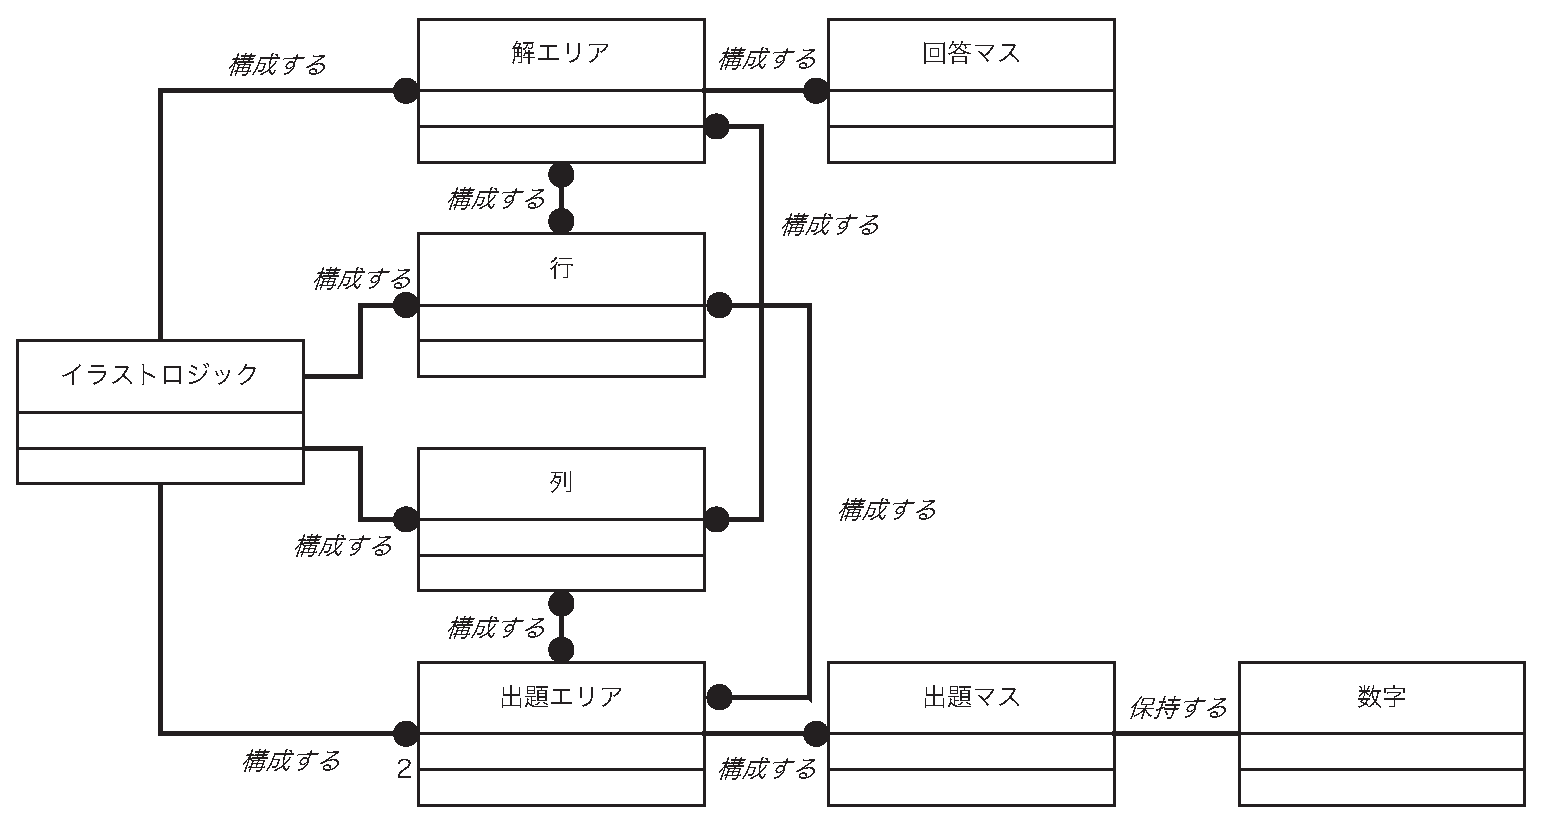
\includegraphics[width=15cm]{./image/class-relation.eps}
\caption{関連を反映させたクラス図}
\label{fig:class-relation}
\end{figure}

\section{操作の洗い出し}
図\ref{fig:class-method}に簡単な操作を書き込んだクラス図を示す。

\begin{figure}[hp]
\centering
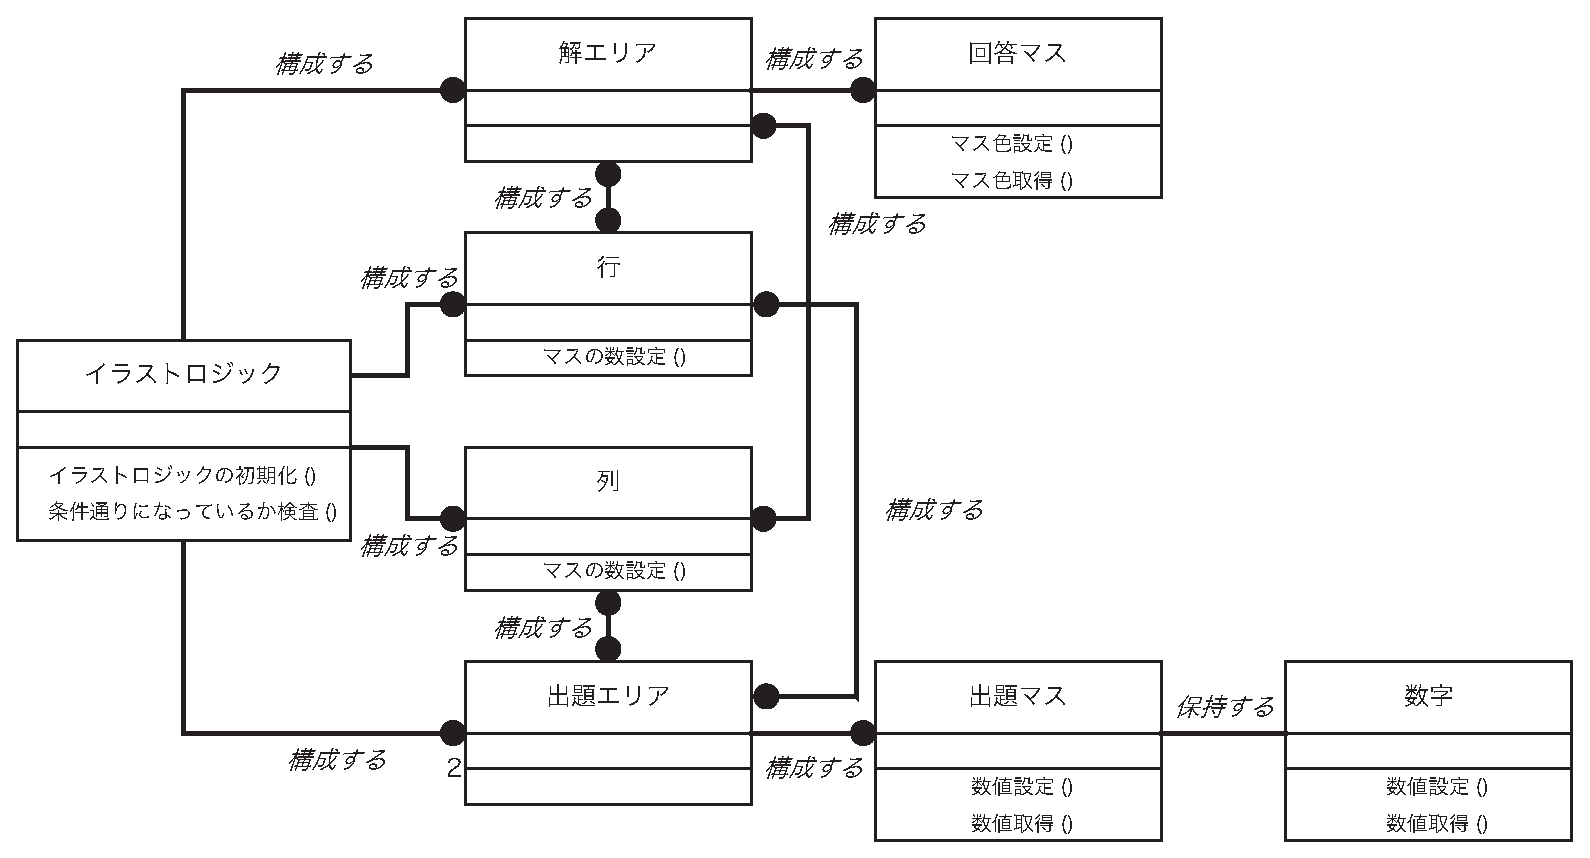
\includegraphics[width=15cm]{./image/class-method.eps}
\caption{簡単な操作を書き込んだクラス図}
\label{fig:class-method}
\end{figure}

\section{属性の洗い出し}
図\ref{fig:class-attribute}に属性を書き込んだクラス図を示す。

\begin{figure}[hp]
\centering
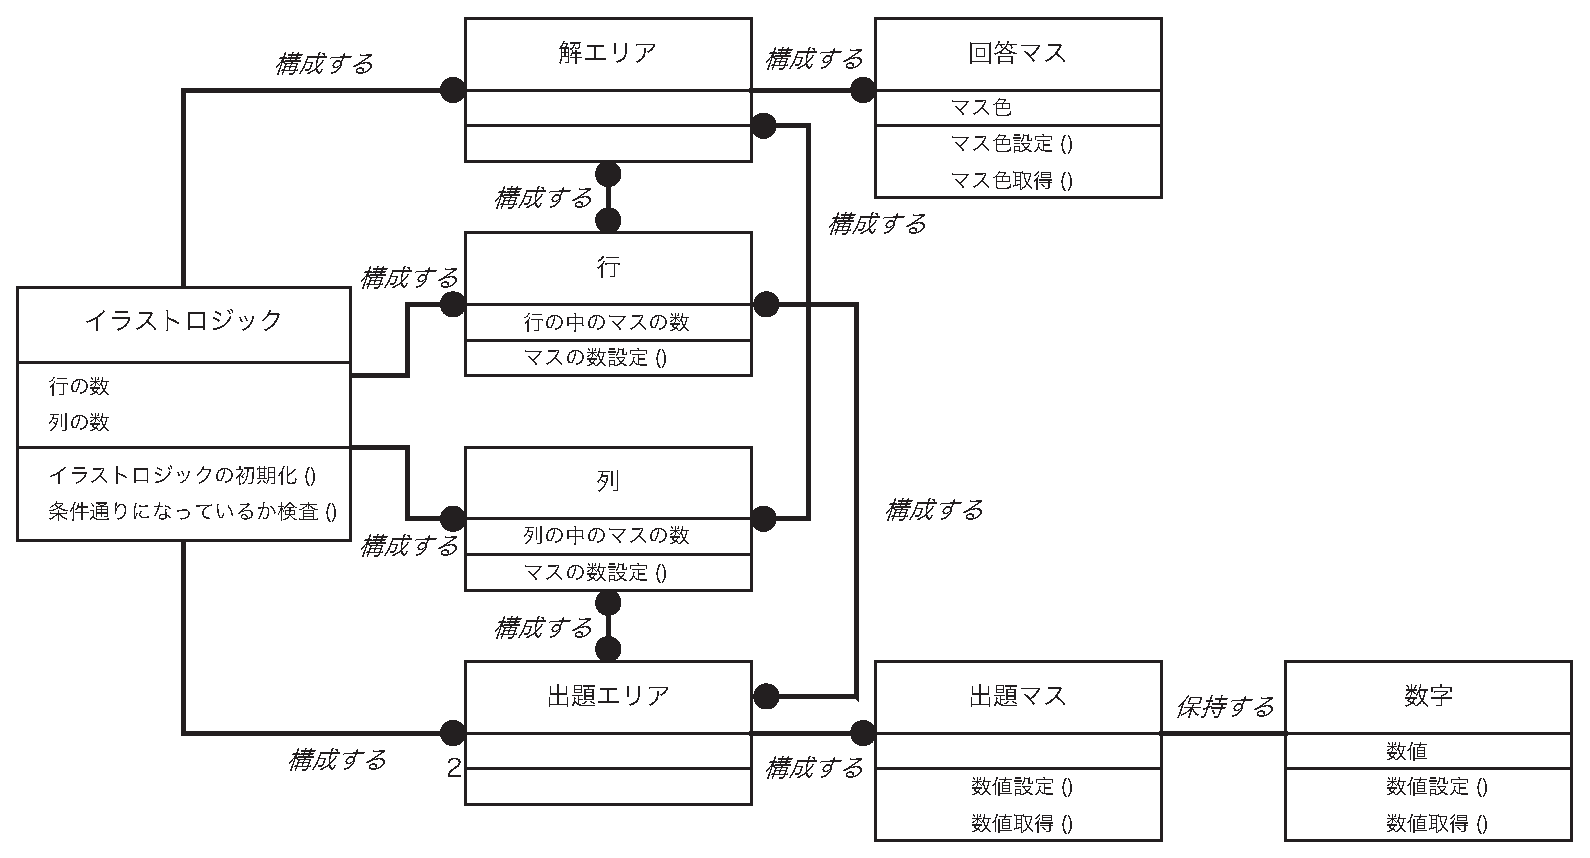
\includegraphics[width=15cm]{./image/class-attribute.eps}
\caption{属性を書き込んだクラス図}
\label{fig:class-attribute}
\end{figure}

\end{document}

